\section{Metoda výroby keramických substrátů (Tape casting)}
- popis procesu, cílové aplikace, typy keramických substrátů a jejich parametry

Tape casting je základní tvářecí metoda používaná pro výrobu tenkých, širokých keramických pásků. Surovinou je keramický prášek, který se smíchá s rozpouštědly a přísadami a vytvoří volně tekoucí licí kaši.

Keramická kaše plynule roztírá po dopravníkovém pásu za pomoci nože, aby se vytvořila rovná, rovnoměrná vrstva. Tato vrstva suspenze se následně vysuší a navine a je připravena k dalšímu zpracování.

Takové pásky se používají např. jako desky plošných spojů v integrovaných vícevrstvých obvodech, např. pro tzv. obvody LTCC (low-temperature co-fired ceramics). 

Výroba integrovaných vícevrstvých obvodů, zejména vícevrstvých LTCC, vyžaduje přísné výrobní tolerance; tendence k závislosti tolerancí na šarži by měla být minimální. Optimalizace výrobního procesu s ohledem na tyto faktory, a tedy i zlepšení kvality a reprodukovatelnosti výrobků, vyžaduje důkladné pochopení jednotlivých kroků procesu a souvisejících ovlivňujících proměnných. Je nezbytné korelovat různé procesní a materiálové parametry s vlastnostmi pásky, které určují konečný výrobek. Prostor parametrů je zde velmi rozsáhlý, a tak například reologické chování licí suspenze lze přičíst interakci mezi jednotlivými složkami suspenze na mikroskopické úrovni. Makroskopické faktory, např. geometrie zařízení nebo rychlost pásu, mají zase vliv jak na tvar pásu, tak na jeho mikrostrukturu.  
\begin{figure}[h]
   \begin{center}
     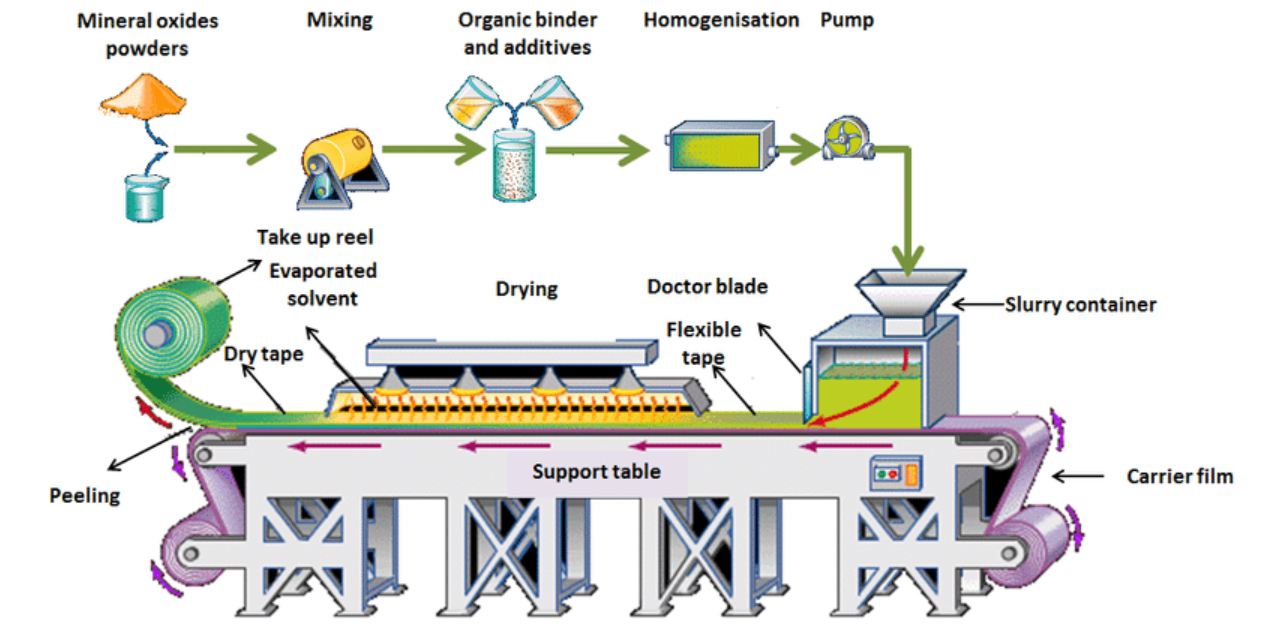
\includegraphics[scale=0.3]{images/Casting.png}
   \end{center}
   \caption{Proces casting tape}
\end{figure}

\subsection{Cílové aplikace}
Používá se k velkovýrobě keramických substrátů (LTCC,Al2O3, BeO)
\subsection{Typy keramických substrátů a jejich parametry}
LTCC,Al2O3, BeO

Dobré tepelné vlastnosti, spolehlivé, vhodné do vyšších teplot, chemicky odolné, odolné= vůči rozdílným klimatům.